\documentclass[11pt,a4paper]{article}

%-------------------------------------
%            Informations Générales
%-------------------------------------

%\NeedsTeXFormat{LaTeX2e}[2009/09/24]
%\ProvidesPackage{style}[2009/09/24 Extension personnelle, V1.0]

%-------------------------------------
% 						extensions
%-------------------------------------
\usepackage[T1]{fontenc} 
\usepackage[utf8]{inputenc}
\usepackage[francais]{babel}
\usepackage{url}
\usepackage{etex}
\usepackage{enumitem}
\usepackage{multicol}
\usepackage{bbm}
\usepackage{amsmath,amsthm,amssymb}
\usepackage[official]{eurosym}
%\usepackage{pifont}
\usepackage[left=1cm, right=1cm, top=1.5cm, bottom=1.5cm]{geometry}
\usepackage{exercise}
\usepackage{graphics}
\usepackage{array,multirow,makecell}
\usepackage{verbatim}
\usepackage[dvipsnames,table]{pstricks}
\usepackage{pstricks-add,pst-plot,pst-text,pst-tree,pst-eps,pst-fill,pst-node,pst-math,pst-blur,pst-func}
\usepackage{pgf,tikz}
\usepackage{tipfr}
\usepackage{thmbox}
\usepackage{calc}
\usepackage{ifthen}
\usepackage{pdfpages}
\usepackage{colortbl}
%\usepackage{sagetex}
\usetikzlibrary{arrows,patterns}
%\input tabvar
\usepackage{tkz-tab}
\usepackage{listings}
\usepackage[np]{numprint}
%\usepackage{tabularx}
\usepackage{fancybox,fancyhdr}
\usepackage{thmtools}
\usepackage{bclogo}
\usepackage{lastpage}

%------------------------------------- 
%        		Abréviations personnelles
%-------------------------------------
\newcommand{\Cc}{\textbf{Conclusion : }}
\newcommand{\DNS}{\textbf{Devoir Non Surveillé}}
\newcommand{\DS}{\textbf{Devoir Surveillé}}
\newcommand\fpsd{une fonction polynôme du second degré~}
\newcommand{\N}{\mathbb{N} } % Raccourci pour l'ensemble des entiers naturels
\newcommand{\R}{\mathbb{R}} % Raccourci pour l'ensemble des réels
\newcommand{\Z}{\mathbb{Z}} % Raccourci pour l'ensemble des entiers relatifs
%\newcommand{\N}{\mathbb{N}} % Raccourci pour l'ensemble des réels

%----------------------------------------------------------------------------------------------- 
% 							Commandes mathématiques
%-----------------------------------------------------------------------------------------------
\renewcommand{\vec}[1]{\overrightarrow{#1}}	% Raccourci pour vecteurs
\newcommand{\inv}[1]{\dfrac{1}{#1}} % Raccourci pour l'inverse des réels
\newcommand{\e}{\text{e}}
\newcommand*{\E}{\ensuremath{\mathrm{e}}}
\newcommand{\lnx}{\ln(x)}

%----------------------------------------------------------------------------------------------- 
% 							Commandes Tableaux
%-----------------------------------------------------------------------------------------------
\setcellgapes{3pt}
\makegapedcells
\newcolumntype{R}[1]{>{\raggedleft\arraybackslash }b{#1}}
\newcolumntype{L}[1]{>{\raggedright\arraybackslash }b{#1}}
\newcolumntype{C}[1]{>{\centering\arraybackslash }b{#1}}

%----------------------------------------------------------------------------------------------- 
% 							Commandes Listes
%-----------------------------------------------------------------------------------------------
% Redéfinition du premier niveau
\renewcommand{\theenumi}{\arabic{enumi}}
\renewcommand{\labelenumi}{\textbf{\theenumi)}}
% Redéfinition du deuxième niveau
\renewcommand{\theenumii}{\alph{enumii}}
\renewcommand{\labelenumii}{\textbf{\theenumii)}}

%-----------------------------------------------------------------------------------------------
%							 		Environnement - Macros
%-----------------------------------------------------------------------------------------------
\setlength{\columnsep}{20pt}
\setlength{\columnseprule}{0.5pt}
\renewcommand{\thesection}{\arabic{section}}
%\renewcommand{\thesection}{\arabic{section}}
%La numérotation des section repart à 0 lorsque l'on change de partie
%\makeatletter\@addtoreset{section}{chapter}\makeatother
\makeatletter\@addtoreset{subsection}{section}\makeatother
%\renewcommand{\thechapter}{\arabic{chapter}}
%\renewcommand{\thesection}{\arabic{section}}
\renewcommand{\thesubsection}{\arabic{subsection}}
%Modifier la section dans son positionnement, sa forme, couleur,...
%\makeatletter
%\renewcommand\section{\@startsection {section}{1}{\z@}%
%                                   {-1.5ex \@plus -0.5ex \@minus -.2ex}%
 %                                  {1.8ex \@plus .2ex}%
  %                                 {\raggedleft\normalfont\color{gray}\large\bfseries}}
%\makeatother
\newenvironment{maliste}%
{ \begin{list}%
	{$\bullet$}%
	{\setlength{\labelwidth}{30pt}%
	 \setlength{\leftmargin}{35pt}%
	 \setlength{\itemsep}{\parsep}}}%
{ \end{list} }


%------------------------------------------------------------------------------------------------
% Paramétrage du langage TI pour la reconnaissance des mots clé utilisés
% A compléter avec les fonctions du catalogue de texas.
%------------------------------------------------------------------------------------------------
\lstdefinelanguage{TI}{%
       morekeywords={%
        %%% CONTROLE.
          If, Then, Else, For, While, Repeat, End, Pause, Lbl, Goto, IS>, DS<, Menu, prgm, Return, Stop, EffVar, GraphStyle,
        %%% ENTREES & SORTIES
          Input, Prompt, Disp, AffGraph, AffTable, Output, codeTouch, EffEcr, EffTable, CaptVar,
        %%% CATALOG
         NbrAléat,
        %%% FONCTIONS NUMERIQUES
          cos, sin, tan, acos, asin, atan,
        %%% CONSTANTES
          pi,
      },
      sensitive=true,
      morecomment=[l]{\#},
      morestring=[b]',
    }


%---------------------------------------------------------------------------------------- 
% 									Environnement NSI
%----------------------------------------------------------------------------------------

\newenvironment{NSI}[2]
{
	\noindent
	\setlength{\fboxsep}{0cm}\setlength{\fboxrule}{0pt}\framebox[19cm]{
		\setlength{\fboxsep}{0.25cm}\setlength{\fboxrule}{1pt}
		\Huge{\textbf{#1 :}}
		\hspace{0.5cm}{\huge{#2}}\hfill
	}
	{\newline \rule[0cm]{\linewidth}{0.05em}}
}

%---------------------------------------------------------------------------------------- 
% 									Environnement de cours
%----------------------------------------------------------------------------------------
\newcounter{nbCrs}
%\setcounter{nbCrs}{1}

\newenvironment{headCrs}[1]
{
	\addtocounter{nbCrs}{1}
	\noindent
	\setlength{\fboxsep}{0cm}\setlength{\fboxrule}{0pt}\framebox[19cm]{
		\setlength{\fboxsep}{0.25cm}\setlength{\fboxrule}{1pt}
		\Ovalbox{\Huge{\textbf{\thenbCrs}}}
		\hspace{0cm plus 1fill}{\huge{\textbf{#1}}}
	}
	{\newline \rule[-0.3cm]{\linewidth}{0.05em}}
}



%-----------------------------------------------------------------------------------------------
% 								Environnement d'Activité
%-----------------------------------------------------------------------------------------------
\newcounter{nbAct}
%\setcounter{nbAct}{1}

\newenvironment{headAct}[1]
{
	\setlength{\fboxsep}{-0.5cm}\setlength{\fboxrule}{0pt} 
	\ifthenelse{\equal{#1}{Activité}}
		{
			\addtocounter{nbAct}{1}
			\noindent
			\framebox[19cm]{
				\begin{Huge}
					$\rhd$ %\hspace{\stretch{1}} 
					\textbf{#1~\thenbAct}
					\hspace{\stretch{1}} %$\bigcirc$
				\end{Huge}			  
			}
		}
		{
			\noindent
			\framebox[19cm]{
				\begin{Huge}
					$\bigcirc$ \hspace{\stretch{1}} 
					\textbf{#1~\thenbAct}
					\hspace{\stretch{1}} $\bigcirc$
				\end{Huge}				  
			}
		}
}
{\newline \rule{\linewidth}{1pt} \medskip}

%-----------------------------------------------------------------------------------------------
% 								Environnement d'AP
%-----------------------------------------------------------------------------------------------
\newcounter{nbAP}

\newenvironment{headAP}[1]
{
	\setlength{\fboxsep}{-0.5cm}\setlength{\fboxrule}{0pt} 
	\ifthenelse{\equal{#1}{Accompagnement Personnalisé}}
		{
			\addtocounter{nbAP}{1}
			\framebox[18cm]{
				\begin{Huge}
					$\square$ \hspace{\stretch{1}} 
					\textbf{#1~\thenbAP}
					\hspace{\stretch{1}} $\square$
				\end{Huge}				  
			}
		}
		{
			\framebox[18cm]{
				\begin{Huge}
					$\square$ \hspace{\stretch{1}} 
					\textbf{#1~\thenbAP}
					\hspace{\stretch{1}} $\square$
				\end{Huge}				  
			}
		}
}
{\newline \rule{\linewidth}{1pt}}

%------------------------------------- 
% 				Environnement Exercices
%-------------------------------------
\newcounter{nbEx}
%\setcounter{nbAct}{1}

\newenvironment{headEx}[1]
{
	\setlength{\fboxsep}{-0.5cm}\setlength{\fboxrule}{0pt} 
	\ifthenelse{\equal{#1}{Exercices}}
		{
			\addtocounter{nbEx}{1}
			\framebox[18cm]{
				\begin{Huge}
					\textbf{#1}
					\hspace{\stretch{1}} \textbf{\thenbEx}
				\end{Huge}				  
			}
		}
		{
			\framebox[18cm]{
				\begin{Huge}
					\textbf{#1}
					\hspace{\stretch{1}} \textbf{\thenbEx}
				\end{Huge}				  
			}
		}
}
{\newline \rule{\linewidth}{1pt}}

%------------------------------------- 
% 				Environnement TP Info
%-------------------------------------
\newcounter{nbTP}

\newenvironment{headTP}[1]
{
	\setlength{\fboxsep}{-0.5cm}\setlength{\fboxrule}{0pt} 
	\ifthenelse{\equal{#1}{TP}}
		{
			\addtocounter{nbTP}{1}
			\framebox[18cm]{
				\begin{Huge}
					\textbf{#1}
					\hspace{\stretch{1}} \textbf{\thenbTP}
				\end{Huge}				  
			}
		}
		{
			\framebox[18cm]{
				\begin{Huge}
					\textbf{#1}
					\hspace{\stretch{1}} \textbf{\thenbTP}
				\end{Huge}				  
			}
		}
}
{\newline \rule{\linewidth}{1pt}}


%------------------------------------- 
% 				Environnement DNS
%-------------------------------------
\newcounter{nbDNS}
%\setcounter{nbDNS}{1}

\newenvironment{headDNS}[4]	%{DNS}{date}{sujet}{classe}
{
	\setlength{\fboxsep}{0.25cm}\setlength{\fboxrule}{0pt} 
	\ifthenelse{\equal{#1}{DNS}}
		{
			\addtocounter{nbDNS}{1}
			\noindent
			\framebox[18.5cm]{
					\LARGE{ \DNS } \textbf{~\thenbDNS} \hspace{\stretch{1}} \large{#2}
			}
			\newline
			\framebox[18.5cm]{
					\makebox[2\width]{\small{#3}} \hspace{\stretch{1}} \makebox[5\width]{\large{#4}}
			}
		}
		{
			%\addtocounter{nbDNS}{1}			
			\noindent
			\framebox[18.5cm]{
					\LARGE{ #1 } \textbf{~\thenbDNS} \hspace{\stretch{1}} \large{#2}
			}
			\newline
			\framebox[18.5cm]{
					\makebox[2\width]{\small{#3}} \hspace{\stretch{1}} \makebox[5\width]{\large{#4}}
			}
		}
}
{\newline \rule{\linewidth}{1pt}}

%------------------------------------- 
% 				Environnement DS
%-------------------------------------
\newcounter{nbDS}
%\setcounter{nbDS}{1}

\newenvironment{headDS}[4]	%{DS}{date}{sujet}{classe}
{
	\setlength{\fboxsep}{0.25cm}\setlength{\fboxrule}{0pt} 
	\ifthenelse{\equal{#1}{DS}}
		{
			\addtocounter{nbDS}{1}
			\noindent
			\framebox[18.5cm]{
					\LARGE{ \DS } \textbf{~\thenbDS} \hspace{\stretch{1}} \large{#2}
			}
			\newline
			\framebox[18.5cm]{
					\makebox[2\width]{\small{#3}} \hspace{\stretch{1}} 	\makebox[2\width]{\large{#4}}
			}
		}
		{
			\noindent
			\framebox[18.5cm]{
					\Large{ #1 } \textbf{~\thenbDS} \hspace{\stretch{1}} \large{#2}
			}
			\newline
			\framebox[18.5cm]{
					\makebox[2\width]{\small{#3}} \hspace{\stretch{1}}\hfill \makebox[5\width]{\large{#4}}
			}
		}
}
{\newline \rule{\linewidth}{1pt}\bigskip}

%------------------------------------- 
% 				Environnement de TEST
%-------------------------------------
\newcounter{nbTEST}
%\setcounter{nbTEST}{1}

\newenvironment{headTEST}[2]	%{Test}{classe}
{
	\setlength{\fboxsep}{0.25cm}\setlength{\fboxrule}{0pt} 
	\ifthenelse{\equal{#1}{TEST}}
		{
			\addtocounter{nbTEST}{1}
			\noindent
			\framebox[18.5cm]{
					\makebox[4cm]{\LARGE{ #1 } \textbf{~\thenbTEST}} \hspace{\stretch{1}} \makebox[8cm][l]{\LARGE{Nom:}}
			}
			\newline
			\framebox[18.5cm]{
					\makebox[4cm]{\large{#2}} \hspace{\stretch{1}} \makebox[8cm][l]{\LARGE{Prénom:}}
			}
		}
		{
			\noindent
			\framebox[18.5cm]{
					\Large{ #1 } \textbf{~\thenbTEST} \hspace{\stretch{1}} \makebox[10cm]{Corrigé}
			}
			\newline
			\framebox[18.5cm]{
					\makebox[6cm]{\small{#2}}
			}
		}
}
{\newline \rule{\linewidth}{1pt}}

%------------------------------------- 
% 				Environnement de ACQUIS
%-------------------------------------
\newcounter{nbACQUIS}
%\setcounter{nbTEST}{1}

\newenvironment{headACQUIS}[2]	%{Test}{classe}
{
	\setlength{\fboxsep}{0.25cm}\setlength{\fboxrule}{0pt} 
	\ifthenelse{\equal{#1}{ACQUIS}}
		{
			\addtocounter{nbACQUIS}{1}
			\noindent
			\framebox[18.5cm]{
					\makebox[4cm]{\LARGE{ #1 } \textbf{~\thenbACQUIS}} \hspace{\stretch{1}} \makebox[8cm][l]{\LARGE{Nom:}}
			}
			\newline
			\framebox[18.5cm]{
					\makebox[4cm]{\large{#2}} \hspace{\stretch{1}} \makebox[8cm][l]{\LARGE{Prénom:}}
			}
		}
		{
			\noindent
			\framebox[18.5cm]{
					\Large{ #1 } \textbf{~\thenbACQUIS} \hspace{\stretch{1}} \makebox[10cm]{Corrigé}
			}
			\newline
			\framebox[18.5cm]{
					\makebox[6cm]{\small{#2}}
			}
		}
}
{\newline \rule{\linewidth}{1pt}}

%------------------------------------- 
% 				Environnement de QCM
%-------------------------------------
\newcounter{nbQCM}
%\setcounter{nbQCM}{1}

\newenvironment{headQCM}[2]	%{QCM}{classe}
{
	\setlength{\fboxsep}{0.25cm}\setlength{\fboxrule}{0pt} 
	\ifthenelse{\equal{#1}{QCM}}
		{
			\addtocounter{nbQCM}{1}
			\noindent
			\framebox[18.5cm]{
					\makebox[4cm]{\LARGE{ #1 } \textbf{~\thenbQCM}} \hspace{\stretch{1}} \makebox[8cm][l]{\LARGE{Nom:}}
			}
			\newline
			\framebox[18.5cm]{
					\makebox[4cm]{\large{#2}} \hspace{\stretch{1}} \makebox[8cm][l]{\LARGE{Prénom:}}
			}
		}
		{
			\noindent
			\framebox[18.5cm]{
					\Large{ #1 } \textbf{~\thenbQCM} \hspace{\stretch{1}} \makebox[10cm]{Corrigé}
			}
			\newline
			\framebox[18.5cm]{
					\makebox[6cm]{\small{#2}}
			}
		}
}
{\newline \rule{\linewidth}{1pt}}



%------------------------------------- 
% 				Environnement de DSSC
%-------------------------------------
\newcounter{nbDSSC}
%\setcounter{nbQCM}{1}

\newenvironment{headDSSC}[2]	%{DSSC}{classe}
{
	\setlength{\fboxsep}{0.25cm}\setlength{\fboxrule}{0pt} 
	\ifthenelse{\equal{#1}{DS}}
		{
			\addtocounter{nbDSSC}{1}
			\noindent
			\framebox[18.5cm]{
					\makebox[4cm]{\LARGE{ #1 } \textbf{~\thenbDSSC}} \hspace{\stretch{1}} \makebox[8cm][l]{\LARGE{Nom:}}
			}
			\newline
			\framebox[18.5cm]{
					\makebox[4cm]{\large{#2}} \hspace{\stretch{1}} \makebox[8cm][l]{\LARGE{Prénom:}}
			}
		}
		{
			\noindent
			\framebox[18.5cm]{
					\Large{ #1 } \textbf{~\thenbDSSC} \hspace{\stretch{1}} \makebox[10cm]{Corrigé}
			}
			\newline
			\framebox[18.5cm]{
					\makebox[6cm]{\small{#2}}
			}
		}
}
{\newline \rule{\linewidth}{1pt}}

%-------------------------------------
% 					Table des matières
%-------------------------------------

\renewcommand{\contentsname}{Sommaire} 


%-------------------------------------
% 					Fin du package
%-------------------------------------

%\endinput


\newcounter{num}
\newcounter{rem}

\begin{document}

\setcounter{num}{0}
\setcounter{rem}{0}
\renewcommand{\arraystretch}{1.25}
%\setlength{\tabcolsep}{0.4cm}
\setlength{\parindent}{0cm}

\newcommand{\Frac}[2]{\displaystyle{\frac{#1}{#2}}}





%\begin{NSI}
%{Activité}{Protocole de routage}
%\end{NSI}

\begin{huge}
\textbf{Activité : } Protocole de routage
\end{huge}\medskip
\hrule

%
%\section*{Passerelle et interface}
%
%Les routeurs sont des appareils munis de plusieurs \textbf{interfaces} réseaux qui permettent aux routeurs de communiquer entre eux. Les interfaces sont désignées par leur nom ou par leur adresse IP. \medskip
%
%Une \textbf{passerelle} est un routeur ou une interface du routeur qui permet d'accéder au réseau de destination.\medskip
%
%Sue la figure ci-dessous, les réseaux L1 et L2 sont reliés par différents routeurs.
%
%\begin{center}
%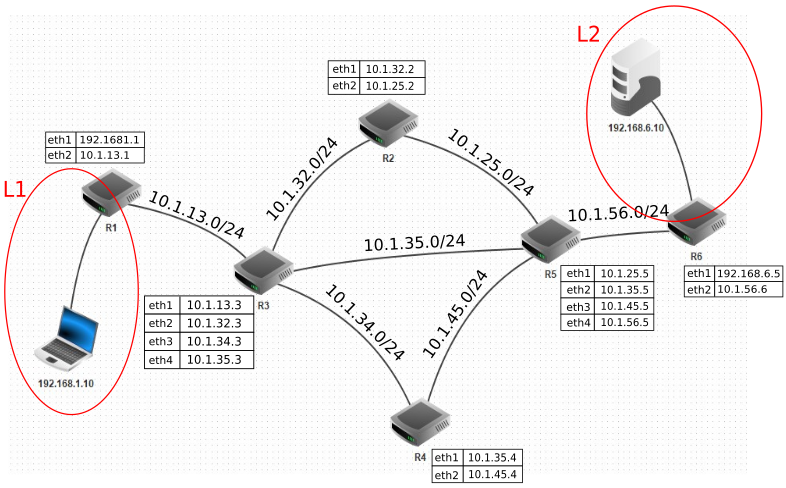
\includegraphics[scale=0.8]{../img/reseau_complet.png}
%\end{center}
%
%%
%%\begin{enumerate}
%%\item Quelles sont les interfaces du routeur R1 ?\vfill
%%\item Quelle est l'interface du routeur R1 pour accéder au réseau L2 ?\vfill
%%\item Quelle est la passerelle suivante du routeur R1 pour accéder au réseau L2 ?\vfill
%%
%%\item Quelles sont les interfaces du routeur R3 ?\vfill
%%\item Le routeur R3 envoie les paquets vers le routeur R5. 
%%
%%Quelle est l'interface utilisée pour accéder au réseau L2 ? Quelle est la passerelle suivante ?\vfill
%%
%%\item Un utilisateur du portable du réseau L1 se connecte sur le serveur du réseau L2. 
%%
%%Quelle est la passerelle renseignée sur le portable ?\vfill
%%
%%\end{enumerate}
%%
%%\newpage
%
%\section*{Table de routage}
%
%Chaque routeur dispose d'une table de routage qui contient les différents réseaux auxquels ils peut accéder, les passerelles à utiliser pour y accéder et les interfaces réseaux à utiliser.
%
%\begin{center}
%\begin{tabular}{*{3}{|C{4cm}}|}\hline
%\textbf{destination} & \textbf{passerelle} & \textbf{interface} \\\hline
%IP destination/masque & routeur ou IP & carte réseau ou IP \\\hline
%\end{tabular}
%\end{center}
%
%
%Au démarrage du réseau, après la mise sous tension, les tables de routage sont vides et chaque routeur commence par identifier ses voisins immédiats et complète sa table.
%
%Après un certain temps, les routeurs échangent leurs informations et les tables se stabilisent.
%
%\begin{enumerate}
%\item Au démarrage, la table de routage du routeur R1 est vide. Compléter sa table avec ses voisins immédiats.
%
%\begin{center}
%\begin{tabular}{*{3}{|C{4cm}}|}\hline
%\textbf{réseau destination} & \textbf{passerelle suivante} & \textbf{interface} \\\hline
% & &  \\\hline
% & &  \\\hline
%\end{tabular}
%\end{center}
%
%\item Au démarrage, la table de routage du routeur R3 est vide aussi. Compléter sa table avec ses voisins immédiats.
%
%\begin{center}
%\begin{tabular}{*{3}{|C{4cm}}|}\hline
%\textbf{destination} & \textbf{passerelle} & \textbf{interface} \\\hline
% & &  \\\hline
% & &  \\\hline
% & &  \\\hline
% & &  \\\hline
%\end{tabular}
%\end{center}
%
%
%\item Les routeurs R1 et R3 échangent leurs tables. Compléter la table de routage du routeur R1 avec les nouvelles informations.
%
%\begin{center}
%\begin{tabular}{*{3}{|C{4cm}}|}\hline
%\textbf{destination} & \textbf{passerelle} & \textbf{interface} \\\hline
% & &  \\\hline
% & &  \\\hline
% & &  \\\hline
% & &  \\\hline
% & &  \\\hline
% & &  \\\hline
%\end{tabular}
%\end{center}
%
%
%
%%\item On donne la table de routage du routeur R3. Compléter les cases vides avec les bonnes valeurs.
%%
%%\begin{center}
%%\begin{tabular}{*{3}{|C{4cm}}|}\hline
%%\textbf{réseau destination} & \textbf{passerelle suivante} & \textbf{interface} \\\hline
%%10.1.13.0/24 & &  \\\hline
%%10.1.32.0/24 & &  \\\hline
%%10.1.34.0/24 & &  \\\hline
%%10.1.35.0/24 & &  \\\hline
%%192.168.1.0/24 & &  \\\hline
%%192.168.6.0/24 & &  \\\hline
%%\end{tabular}
%%\end{center}
%
%%Que peut-on dire concernant la dernière route de la table ?\vspace{2cm}
%
%\item Après de multiples échanges entre les routeurs, les tables de routage se stabilisent. Compléter la table de routage du routeur R1 une fois stabilisée.
%
%\begin{center}
%\begin{tabular}{*{3}{|C{4cm}}|}\hline
%\textbf{destination} & \textbf{passerelle} & \textbf{interface} \\\hline
% & &  \\\hline
% & &  \\\hline
% & &  \\\hline
% & &  \\\hline
% & &  \\\hline
% & &  \\\hline
% & &  \\\hline
% & &  \\\hline
%\end{tabular}
%\end{center}
%
%\end{enumerate}


%\newpage


%\section*{Protocoles}

%Sur la figure ci-dessous, les réseaux L1 et L2 sont reliés par différents routeurs.

\begin{center}
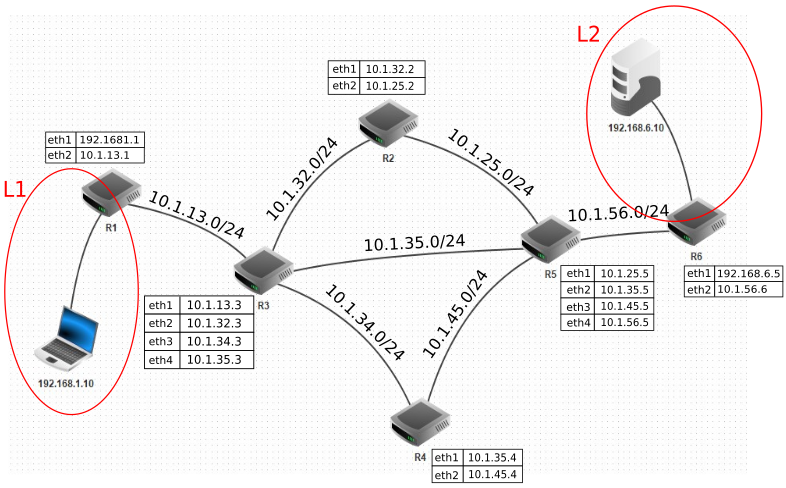
\includegraphics[scale=0.84]{../img/reseau_complet.png}
\end{center}

Les tables de routage disposent des différentes routes pour accéder à d'autres réseaux, mais en l'état, un paquet de données envoyé par une machine du réseau L1 vers le serveur du réseau L2 ne sait pas quelle route suivre. 

Pour déterminer une route, les routeurs utilisent des protocoles afin de déterminer la meilleure route à suivre.

Il existe plusieurs protocoles. On va en étudier 2 : \textbf{RIP} et \textbf{OSPF}.


\subsection*{Protocole RIP}

Le protocole RIP détermine la meilleure route entre 2 réseaux en mémorisant le nombre de routeurs à traverser pour parvenir au réseau de destination. Cette quantité de routeurs à traverser est appelée \textbf{distance} ou \textbf{métrique}. Cette métrique est enregistrée dans la table de routage.


\begin{enumerate}
\item On donne la table de routage du routeur R6. Compléter la métrique de chaque route avec la bonne valeur.

\begin{center}
\begin{tabular}{*{4}{|C{4cm}}|}\hline
\textbf{destination} & \textbf{passerelle} & \textbf{interface}  & \textbf{distance / métrique} \\\hline
192.168.6.0/24 &  & eth 1 & \\\hline
10.1.56.0/24 &  & eth2 &  \\\hline
10.1.25.0/24 & 10.1.56.5 / R5 & eth2 &  \\\hline
10.1.35.0/24 & 10.1.56.5 / R5 & eth2 &  \\\hline
10.1.45.0/24 & 10.1.56.5 / R5 & eth2 & \\\hline
10.1.34.0/24 & 10.1.56.5 / R5 & eth2 &  \\\hline
10.1.32.0/24 & 10.1.56.5 / R5 & eth2 &  \\\hline
10.1.13.0/24 & 10.1.56.5 / R5 & eth2 &  \\\hline
192.168.1.0/24 & 10.1.56.5 / R5 & eth2 &  \\\hline
\end{tabular}
\end{center}


\item On donne la table de routage du routeur R5. Compléter la métrique de chaque route avec la bonne valeur.

\begin{center}
\begin{tabular}{*{4}{|C{4cm}}|}\hline
\textbf{destination} & \textbf{passerelle} & \textbf{interface}  & \textbf{distance / métrique} \\\hline
10.1.25.0/24 &  & eth1 &  \\\hline
10.1.35.0/24 &  & eth2 &  \\\hline
10.1.45.0/24 &  & eth3 & \\\hline
10.1.56.0/24 &  & eth4 &  \\\hline
10.1.34.0/24 & 10.1.45.4 / R4 & eth3 &  \\\hline
10.1.32.0/24 & 10.1.25.2 / R2 & eth1 &  \\\hline
10.1.13.0/24 & 10.1.35.3 / R3 & eth2 &  \\\hline
192.168.1.0/24 & 10.1.35.3 / R3 & eth2 &  \\\hline
192.168.6.0/24 & 10.1.56.6 / R6 & eth4 & \\\hline
\end{tabular}
\end{center}


\item Après un redémarrage du routeur R3, celui-ci reçoit en premier les informations de la table du routeur R5. Quelles sera alors le contenu de la table de routage du routeur R3.

\begin{center}
\begin{tabular}{*{4}{|C{4cm}}|}\hline
\textbf{réseau destination} & \textbf{passerelle suivante} & \textbf{interface} & \textbf{distance / métrique} \\\hline
 & & & \\\hline
 & & & \\\hline
 & & & \\\hline
 & & & \\\hline
 & & & \\\hline
 & & & \\\hline
 & & & \\\hline
 & & & \\\hline
 & & & \\\hline
\end{tabular}
\end{center}

\item Le routeur R1 envoie sa table de routage au routeur R3. Quelles sont les modifications qui seront effectuées dans la table du routeur R3?

\vspace{2cm}

\item Quelle sera la route suivie par le paquet de données envoyé du réseau L1 au réseau L2 ? Justifier et donner le coût de cette route.



\end{enumerate}
%Dans notre réseau, chaque routeur dispose d'une table de routage qui contient les informations sur les routeurs avec lesquels il communique. La table de routage est mise à jour régulièrement et se complète en deux temps.\medskip
%
%Dans un premier temps, chaque routeur complète sa table de routage avec ses voisins immédiats. Il mémorise les réseaux directement relié à lui, les interfaces utilisées puis met chaque distance à 1.\smallskip
%
%Ensuite, il échange régulièrement sa table avec ses voisins et complète ou met à jour sa table de routage avec les informations détenues par les routeurs voisins.\smallskip
%
%De proche en proche, la table de routage d'un routeur se stabilise et le routeur finit par disposer des informations sur tout le réseau.
%
%Lorsqu'un routeur reçoit les informations d'un routeur voisin, il suit les 4 règles du protocole RIP:
%\begin{itemize}
%\item Il découvre une nouvelle route inconnue vers un sous réseau inconnu, il l' ajoute à sa table;
%\item Il découvre une route plus courte vers un sous-réseau connu, mais passant par un nouveau routeur. L'ancienne route est remplacée par la nouvelle;
%\item Il reçoit une nouvelle route plus longue vers un sous-réseau connu, il l'ignore;
%\item Il reçoit une route plus longue vers un routeur passant par le même voisin, cela signifie qu'un problème est survenu sur l'ancienne route. Il met à jour sa table avec cette nouvelle route. \medskip
%
%Lorsqu'un routeur reçoit une route, il faut augmenter la distance de 1, soit pour la comparer aux autres routes, soit pour l'ajouter à sa table. Les distances indiquent le nombre de routeurs traversés pour accéder à un sous réseau. Lorsque la distance est supérieure à 15, la route est effacée de la table.
%\end{itemize}


%\begin{enumerate}
%%\item Initialiser la table de routage du routeur R1.
%%
%%\begin{center}
%%\begin{tabular}{*{4}{|C{3cm}}|}\hline
%%\textbf{destination} & \textbf{passerelle} & \textbf{interface} & \textbf{distance}\\\hline
%%& & & \\\hline
%%& & & \\\hline
%%\end{tabular}
%%\end{center}
%
%\item Initialiser la table de routage du routeur R3.
%
%\begin{center}
%\begin{tabular}{*{4}{|C{3cm}}|}\hline
%\textbf{destination} & \textbf{passerelle} & \textbf{interface} & \textbf{distance}\\\hline
%& & & \\\hline
%& & & \\\hline
%& & & \\\hline
%& & & \\\hline
%\end{tabular}
%\end{center}
%
%
%\item Une demande RIP intervient, les routeurs s'échangent donc leurs tables avec les routeurs voisins immédiats.
%Compléter la table de routage de R1.
%
%\begin{center}
%\begin{tabular}{*{4}{|C{3cm}}|}\hline
%\textbf{destination} & \textbf{passerelle} & \textbf{interface} & \textbf{distance}\\\hline
%& & & \\\hline
%& & & \\\hline
%& & & \\\hline
%& & & \\\hline
%& & & \\\hline
%& & & \\\hline
%& & & \\\hline
%\end{tabular}
%\end{center}
%
%
%\end{enumerate}

\newpage


\subsection*{Protocole OSPF}

Le protocole RIP ne tient pas compte du débit et de la distance entre les routeurs. De plus, les protocoles RIP ne sont pas adaptés pour les grands réseaux supérieurs à 15 sauts. Le protocole OSPF palie à ces problèmes.\medskip

Ce protocole permet de gérer de grands domaines et prend en compte les débits pour mesurer la rapidité d'une route, son \textbf{coût}. Le calcul du coût se fait avec la relation suivante :
$$\text{c} = \dfrac{10^8}{\text{d}}$$
où \textbf{c} est le coût et \textbf{d} le débit de la route en bits par seconde. A noter que le nombre $10^{8}$ est une constante liée au routeur et peut être différente.
\medskip

Pour simplifier le réseau, on le représente par un graphe:
\begin{itemize}
\item Chaque sommet du graphe représente un routeur;
\item Chaque arête du graphe représente un lien entre deux routeurs;
\item Le poids donné pour chaque arête indique le \textbf{coût} de communication entre 2 routeurs.
\end{itemize}

\begin{center}
\psset{unit=1cm}
\begin{pspicture}(10,6)
\cnodeput(0.5,3.5){R1}{R1}
\cnodeput(5.5,5.5){R2}{R2}
\cnodeput(2.5,3){R3}{R3}
\cnodeput(5,1){R4}{R4}
\cnodeput(7.5,3){R5}{R5}
\cnodeput(9.5,2.5){R6}{R6}
\ncline{R1}{R3}\ncput*{\bf ...}
\ncline{R3}{R2}\ncput*{\bf 4}
\ncline{R3}{R4}\ncput*{\bf 5}
\ncline{R3}{R5}\ncput*{\bf 6}
\ncline{R2}{R5}\ncput*{\bf 3}
\ncline{R4}{R5}\ncput*{\bf ...}
\ncline{R5}{R6}\ncput*{\bf 1}
\end{pspicture}
\end{center} 

\begin{enumerate}
\item Sachant que le débit entre les routeurs R1 et R2 est de 50 Mbits par seconde, calculer le coût de cette route. \vspace{2cm}

\item Calculer le débit de la route qui relie les routeurs R3 et R4.
\vspace{2cm}

\item La communication entre les routeurs R4 et R5 est de 1Gb/s. Calculer son coût. \vspace{2cm}

\item Quelle est la route qui est la plus rapide entre les routeurs R1 et R6 ?
\end{enumerate}

%\subsubsection*{Algorithme de Dijkstra}
%
%\renewcommand\arraystretch{1.8}
%\begin{center}
%\begin{tabular}{*{6}{|C{1.5cm}}|C{2.5cm}|}\hline 
%R1 & R2 & R3 & R4 & R5 & R6 & Sommet fixé\\ \hline
%$0$ & $\infty$ & $\infty$ & $\infty$ & $\infty$ & $\infty$ & R1(0)\\ \hline
%&&&&&&\\ \hline 
%&&&&&&\\ \hline 
%&&&&&&\\ \hline 
%&&&&&&\\ \hline 
%&&&&&&\\ \hline 
%\end{tabular} 
%\end{center}		


%\newpage
%\subsubsection*{Réseau augmenté}
%
%Deux liaisons supplémentaires sont ajoutées au réseau entre les routeurs R1 et R2 d'une part et entre les routeurs R4 et R6 d'autre part. Le réseau est représenté par le graphe suivant:
%
%\begin{center}
%\psset{unit=1cm}
%\begin{pspicture}(10,6)
%\cnodeput(0.5,3.5){R1}{R1}
%\cnodeput(5.5,5.5){R2}{R2}
%\cnodeput(2.5,3){R3}{R3}
%\cnodeput(5,1){R4}{R4}
%\cnodeput(7.5,3){R5}{R5}
%\cnodeput(9.5,2.5){R6}{R6}
%\ncline{R1}{R3}\ncput*{\bf 2}
%\ncline{R1}{R2}\ncput*{\bf 4}
%\ncline{R3}{R2}\ncput*{\bf 4}
%\ncline{R3}{R4}\ncput*{\bf 6}
%\ncline{R3}{R5}\ncput*{\bf 5}
%\ncline{R2}{R5}\ncput*{\bf 2}
%\ncline{R4}{R5}\ncput*{\bf 1}
%\ncline{R4}{R6}\ncput*{\bf 3}
%\ncline{R5}{R6}\ncput*{\bf 5}
%\end{pspicture}
%\end{center} 
%
%En appliquant l'algorithme de Dijkstra, déterminer la route la moins coûteuse entre les routeurs R1 et R6.
%
%\renewcommand\arraystretch{1.8}
%\begin{center}
%\begin{tabular}{*{6}{|C{1.5cm}}|C{2.5cm}|}\hline 
%R1 & R2 & R3 & R4 & R5 & R6 & Sommet fixé\\ \hline
%$0$ & $\infty$ & $\infty$ & $\infty$ & $\infty$ & $\infty$ & R1(0)\\ \hline
%&&&&&&\\ \hline 
%&&&&&&\\ \hline 
%&&&&&&\\ \hline 
%&&&&&&\\ \hline 
%&&&&&&\\ \hline 
%\end{tabular} 
%\end{center}		


\end{document}
